\documentclass{scrartcl}
\usepackage{amsmath,amssymb,graphicx,wrapfig,ulem,qtree}
\usepackage{tikz}
\usetikzlibrary{trees,arrows,automata}
\setkomafont{disposition}{\normalfont\bfseries}

\title{Toy Design Problem}
\subtitle{Foundations of Computer Science - Final Assignment}
\author{Kenny Roffo}

\begin{document}

\maketitle

The diagram below is my original design of this Finite State Machine. The transitions represent which tube the ball is placed in (0 or 1) and the tube the ball exits through ($A$ or $B$). The states represent which direction the levers are facing, in order. This means a state of LRL represents the Levers 1 and 3 being oriented left, and Lever 2 being oriented right.

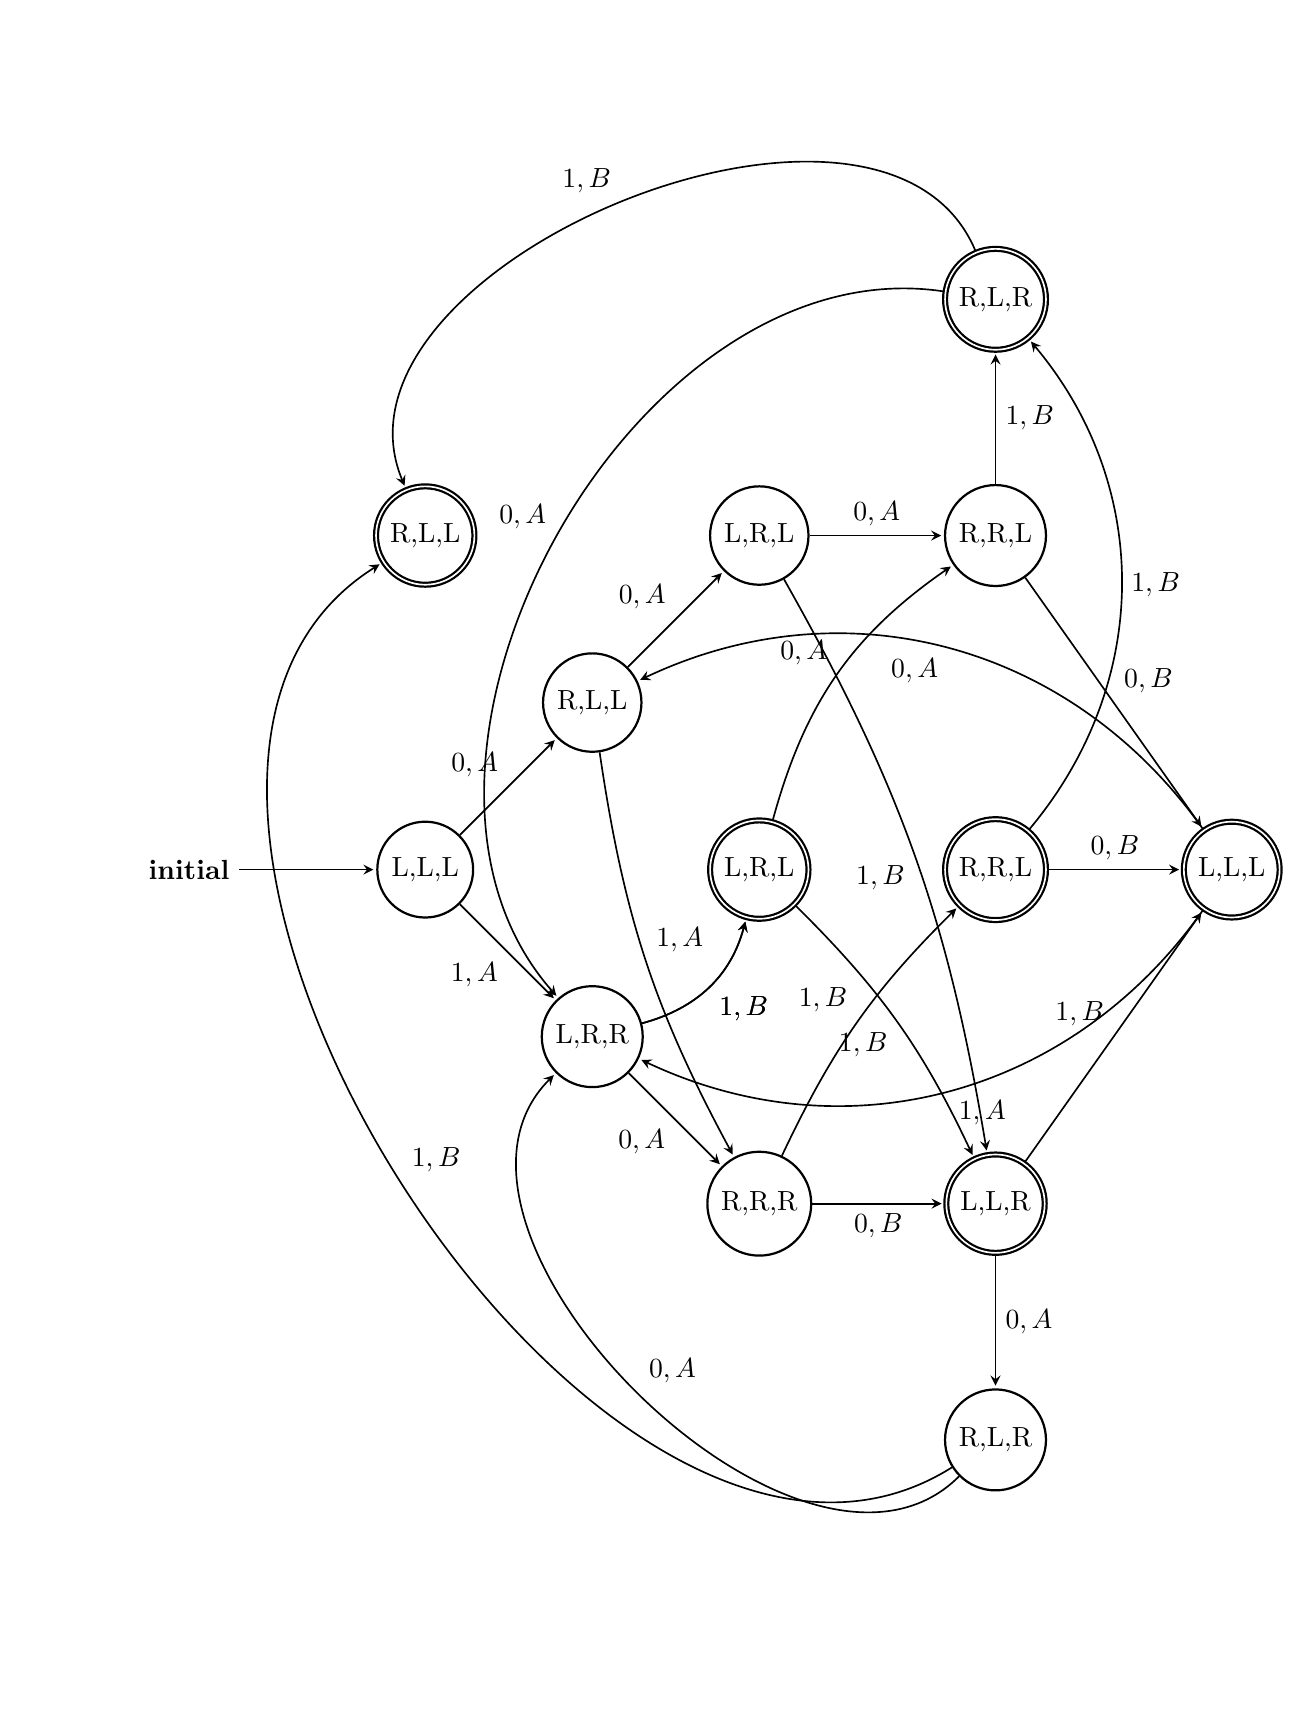
\begin{tikzpicture}
        [
            > = stealth, % arrow head style
            shorten > = 1pt, % don't touch arrow head to node
            auto,
            node distance = 3cm, % distance between nodes
            semithick % line style
        ]
        \tikzstyle{every state}=[
            draw = black,
            thick,
            fill = white,
            minimum size = 4mm
        ]

        \node (initial) {\textbf{initial}};
        \node[state] (LLL) [right of=initial] {L,L,L};
        \node[state] (RLL) [above right of=LLL] {R,L,L};
        \node[state] (LRR) [below right of=LLL] {L,R,R};
        \node[state] (LRL) [above right of=RLL] {L,R,L};
        \node[state, accepting] (LRLf) [below right of=RLL] {L,R,L};
        \node[state] (RRR) [below right of=LRR] {R,R,R};
        \node[state] (RRL) [right of=LRL] {R,R,L};
        \node[state, accepting] (RRLf) [right of=LRLf] {R,R,L};
        \node[state, accepting] (LLR) [right of=RRR] {L,L,R};
        \node[state, accepting] (RLRf) [above of=RRL] {R,L,R};
        \node[state, accepting] (LLLf) [right of=RRLf] {L,L,L};
        \node[state] (RLR) [below of=LLR] {R,L,R};
        \node[state, accepting] (RLLf) [above left of=RLL] {R,L,L};
        
        \path[->] (initial) edge node {} (LLL);
        \path[->] (LLL) edge node {$0,A$} (RLL);
        \path[->, swap] (LLL) edge node {$1,A$} (LRR);
        \path[->] (RLL) edge node {$0,A$} (LRL);
        \path[->, bend right=10] (RLL) edge node {$1,A$} (RRR);
        \path[->, bend right=30, swap] (LRR) edge node {$1,B$} (LRLf);
        \path[->, swap] (LRR) edge node {$0,A$} (RRR);
        \path[->] (LRL) edge node {$0,A$} (RRL);
        \path[->, bend left=10, swap] (LRL) edge node {$1,B$} (LLR);
        \path[->, bend left=20] (LRLf) edge node {$0,A$} (RRL);
        \path[->, bend left=10, swap] (LRLf) edge node {$1,B$} (LLR);
        \path[->, bend left=10] (RRR) edge node {$1,B$} (RRLf);
        \path[->, swap] (RRR) edge node {$0,B$} (LLR);
        \path[->, bend right=30, swap] (LRR) edge node {$1,B$} (LRLf);
        \path[->] (RRL) edge node {$0,B$} (LLLf);
        \path[->, swap] (RRL) edge node {$1,B$} (RLRf);
        \path[->] (RRLf) edge node {$0,B$} (LLLf);
        \path[->, bend right=40, swap] (RRLf) edge node {$1,B$} (RLRf);
        \path[->] (LLR) edge node {$0,A$} (RLR);
        \path[->] (LLR) edge node {$1,B$} (LLLf);
        \path[->, bend left=90, swap] (RLR) edge node {$0,A$} (LRR);
        \path[->, bend left=90, swap] (RLR) edge node {$1,B$} (RLLf);
        \path[->, bend right=70, swap] (RLRf) edge node {$0,A$} (LRR);
        \path[->, bend right=90, swap] (RLRf) edge node {$1,B$} (RLLf);
        \path[->, bend left=40] (LLLf) edge node {$1,A$} (LRR);
        \path[->, bend right=40] (LLLf) edge node {$0,A$} (RLL);
    \end{tikzpicture}

The 
\end{document}
